\section{Auswertung}
\label{sec:Auswertung}

\subsection{Bestimmung der Reichweite von Alphastrahlung}
\subsubsection*{Mittlere Reichweite}
Es wurde eine Messung bei einem Abstand von $30$mm sowie eine zweite bei $36$mm zwischen 
Strahlungsquelle und Halbleiter-Detektor durchgeführt. 
Die aufgenommenen Werte sind in xxx einzusehen.
Wie in \autoref{fig:reichweite} dargestellt, werden die Zählraten gegen die effektive Länge 
aufgetragen.\\
Die horizontalen Geraden schneiden die jweiligen Kurven auf Höhe ihres halben
Maximums. Zudem wird durch den nahezu linear absteigenden Teil der Messwerte eine 
Ausgleichsgerade gelegt. Dafür wird eine lineare Regression durch \cite{numpy} durchgeführt. Die 
dazugehörige Geradengleichung lautet
\begin{equation}
  y = mx + b.
  \label{eq:linreg}
\end{equation}\\
Letztere ergibt die Geradenparameter
\begin{eqnarray}
  m_{\mathrm{30mm}} &=&  -6054,6  \nonumber  \\
  b_{\mathrm{30mm}} &=&  180363,5 \nonumber  \\
  m_{\mathrm{36mm}} &=&  -5903,2  \nonumber  \\
  b_{\mathrm{36mm}} &=&  166936,8 \nonumber
\end{eqnarray}
für die Geraden in \autoref{fig:reichweite}.\\
Die x-Koordinate des Schnittpunkts der Horizontalen und der Ausgleichsgerade markiert die 
mittlere Reichweite der $\alpha$-Teilchen. 
Sie werden zu 
\begin{eqnarray}
  x_{\mathrm{30mm}} &=&   \nonumber  \\
  x_{\mathrm{36mm}} &=&    \nonumber  
\end{eqnarray}
ermittelt.
Wird diese mittlere Reichweite in xxx eingesetzt, können die Energien 
\begin{eqnarray}
  E_{\mathrm{30mm}} &=&   \nonumber  \\
  E_{\mathrm{36mm}} &=&    \nonumber  
\end{eqnarray}
der Teilchen berechnet werden. 


\subsubsection*{Energieverlust}
Wird die Energie der $\alpha$-Teilchen als Funktion der effektiven Länge 
graphisch aufgetragen und eine lineare Regression wie in \autoref{eq:linreg} durchgeführt,
ist die Steigung der Ausgleichsgerade gleich dem Energieverlust $-\frac{dE}{dx}$.
Mit Hilfe von python ergebn sich die Geradenparameter zu \autoref{fig:xxx} und \autoref{fig:xxx}
zu
\begin{eqnarray}
  m_{\mathrm{30mm}} &=&   \nonumber  \\
  b_{\mathrm{30mm}} &=&   \nonumber  \\
  m_{\mathrm{36mm}} &=&   \nonumber  \\
  b_{\mathrm{36mm}} &=&  . \nonumber
\end{eqnarray}


\subsection{Statistik des radioaktiven Zerfalls}
Zunächst werden mit Hilfe von python \cite{numpy} der Mittelwert zu $\mu = 4038,17$ sowie die Standardabweichung von
$\sigma = 134,35$ berechnet. 
Von diesen Werten ausgehend können dann die vergleichbaren Poisson- und Gaußverteilungen 
bestimmt werden.\\
Diese sind zusammen mit den gemessenen Werten in \autoref{fig:hist} aufgetragen.

\begin{figure}
  \centering
  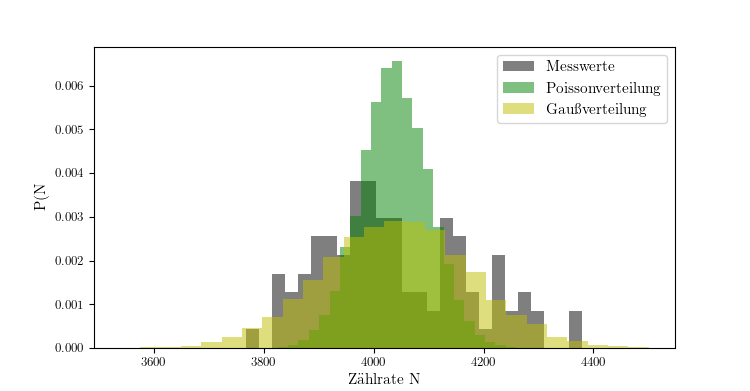
\includegraphics{content/histogramm.png}
  \caption{Die Zerfallsraten im Histogramm aufgetragen im Vergleich zu einer
  Poisson- und einer Gaußverteilung.}
  \label{fig:hist}
\end{figure}


